\section{The Renderers}
\label{sec:renderers}

\subsection{General}

\subsubsection{Reproduction Setups}
\label{sec:reproduction_setups}

The geometry of the actual reproduction setup is specified in
\texttt{.asd} files, just like sound scenes. By default, it is loaded from the
file \texttt{/usr/local/share/ssr/default\_setup.asd}.
Use the \texttt{--setup} command line option to load another reproduction setup file.
Note that the
loudspeaker setups have to be convex. This is not checked by the SSR.
The loudspeakers appear at the outputs of your sound card in the same
order as they are specified in the \texttt{.asd} file, starting with channel 1.

\noindent A sample reproduction setup description:

\begin{verbatim}
<?xml version="1.0"?>
<asdf version="0.1">
  <header>
    <name>Circular Loudspeaker Array</name>
  </header>
  <reproduction_setup>
    <circular_array number="56">
      <first>
        <position x="1.5" y="0"/>
        <orientation azimuth="-180"/>
      </first>
    </circular_array>
  </reproduction_setup>
</asdf>
\end{verbatim}

\noindent We provide the following setups in the directory
\verb+data/reproduction_setups/+:
\begin{itemize}
\item[-] \texttt{2.0.asd}: standard stereo setup at 1.5 mtrs distance
\item[-] \texttt{2.1.asd}: standard stereo setup at 1.5 mtrs distance plus subwoofer
\item[-] \texttt{5.1.asd}: standard 5.1 setup on circle with a diameter of 3 mtrs
\item[-] \texttt{rounded\_rectangle.asd}: Demonstrates how to combine circular
	arcs and linear array segments.
\item[-] \texttt{circle.asd}: This is a circular array of 3 mtrs diameter
	composed of 56 loudspeakers.
\item[-] \texttt{loudspeaker\_setup\_with\_nearly\_all\_features.asd}: This
	setup describes all supported options, open it with your favorite text
	editor and have a look inside.
\end{itemize}

\noindent Note that outputs specified as subwoofers receive a signal having
full bandwidth.
There is some limited freedom in assigning channels to loudspeakers:
If you insert the element \texttt{<skip number="5"/>},
the specified number of output channels are skipped and the following
loudspeakers get higher channel numbers accordingly.

Of course, the binaural and BRS renderers do not load a loudspeaker setup. By
default, they assume the listener to reside in the coordinate origin looking
straight forward.

\subsubsection{A Note on the Timing of the Audio Signals}

The WFS renderer is the only renderer in which the timing of the audio signals is 
somewhat peculiar. None of the other renderers imposes any algorithmic delay on 
individual source signals. Of course, if you use a renderer which is convolution 
based such as the BRS renderer, the employed HRIRs do alter the timing of the 
signals due to their inherent properties. 

This is different with the WFS renderer. Here, also the propagation duration of 
sound from the position of the virtual source to the loudspeaker array is 
considered. That means that the farther a virtual source is located, the longer
is the delay imposed on its input signal. This also holds true for plane waves: 
Theoretically, plane waves do originate from infinity. Though, the SSR does consider
the origin point of the plane wave which is specified in ASDF. This origin point 
also specifies the location of the symbol which represents the respective plane
wave in the GUI. 

We are aware that this procedure can cause confusion and reduces the ability of
a given scene of translating well between different types of renderers. In the 
upcoming version~0.4 of the SSR we will implement an option that will allow you 
specifying for each individual source whether the propagation duration of sound 
shall be considered by a renderer or not. 

\subsubsection{Distance Attenuation}

Note that in all renderers -- except the BRS renderer -- distance attenuation
is handled as $\nicefrac{1}{r}$ with respect to the distance $r$ of the
respective virtual source to the reference position. Sources closer than 0.5
mtrs to the reference position do not experience any increase of amplitude.
Virtual plane waves do not experience any algorithmic distance attenuation in
any renderer.
In future versions of the SSR more freedom in specifying the distance attenuation 
will be provided.

The amplitude reference distance, i.e.~the distance from the reference at which
plane waves are as loud as the other source types (like point sources), can be
set in the SSR configuration file (Section~\ref{sec:ssr_configuration_file}).
The desired amplitude reference distance for a given sound scene can be
specified in the scene description (Section~\ref{sec:asdf}). The default value
is 3~m.

\subsubsection{Doppler Effect}

In the current version of the SSR the Doppler Effect in moving sources is not
supported by any of the renderers.

\subsubsection{Signal Processing}

All rendering algorithms are implemented on a frame-wise basis with an internal
precision of 32 bit floating point. The signal processing is illustrated in
Fig.~\ref{fig:signal_processing}.

The input signal is divided into individual frames of size \emph{nframes}, whereby
\emph{nframes} is the frame size with which JACK is running. Then e.g.\ frame number
$n+1$ is processed both with previous rendering parameters $n$ as well as with
current parameters $n+1$. It is then crossfaded between both processed frames
with cosine-shaped slopes. In other words the effective frame size of the
signal processing is $2\cdot\text{\emph{nframes}}$ with 50\% overlap. Due to the fade-in of
the frame processed with the current parameters $n+1$, the algorithmic latency
is slightly higher than for processing done with frames purely of size
\emph{nframes} and no crossfade.

\begin{figure}
\footnotesize \psfrag{input}{\bf input signal} \psfrag{output}{\bf
output signal} \psfrag{dots}{\bf \dots} \psfrag{+}{\bf +}
\psfrag{n}{frame $n$} \psfrag{n+1}{frame $n\!+\!1$}
\psfrag{n+2}{frame $n\!+\!2$} \psfrag{n+3}{frame $n\!+\!3$}
\psfrag{pn-1}{parameters $n\!-\!1$} \psfrag{pn}{parameters $n$}
\psfrag{pn+1}{parameters $n\!+\!1$} \psfrag{pn+2}{parameters
$n\!+\!2$} \psfrag{pn+3}{parameters $n\!+\!3$}
\hfill
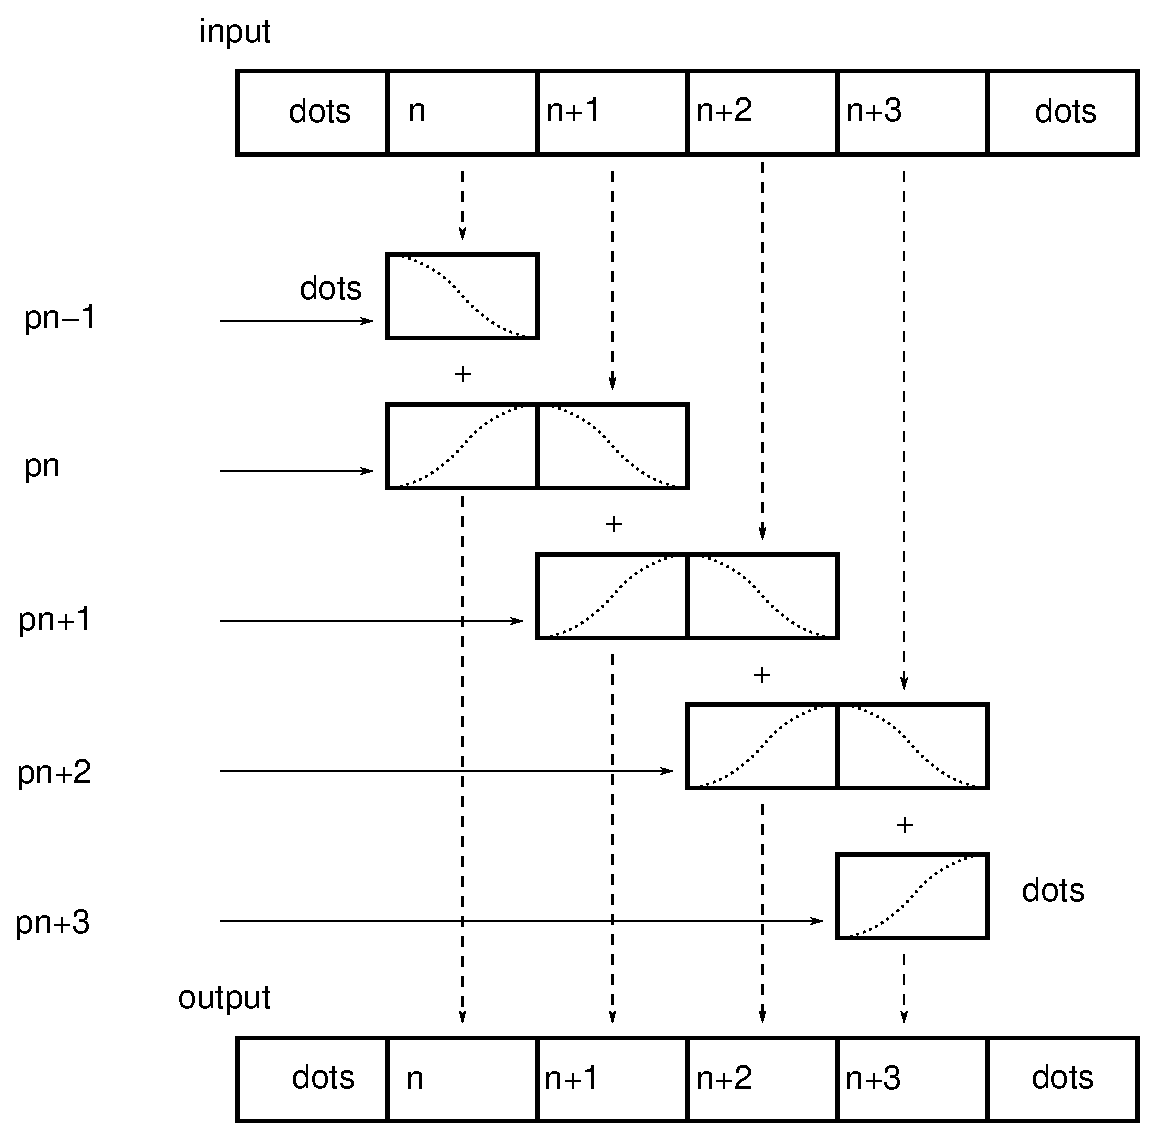
\includegraphics[width=.95\linewidth]{signal_processing}
\caption{\label{fig:signal_processing}{Illustration of the
frame-wise signal processing as implemented in the SSR renderers
(see text).}}
\end{figure}

The implementation approach described above is one version of the standard way
of implementing time-varying audio processing. Note however that this means
that with \emph{all} renderers, moving sources are not physically correctly
reproduced. The physically correct reproduction of moving virtual sources as in
\cite{Ahrens08:MOVING_AES,Ahrens08:SUPERSONIC_AES} requires a different
implementation approach which is computationally significantly more costly.

\subsection{Binaural Renderer}
\label{sec:binaural_renderer}

Binaural rendering is a technique where the acoustical influence of the human
head is electronically simulated to position virtual sound sources in space.
{\bf Be sure that you use headphones to listen.} Note that the current binaural
renderer reproduces all virtual sources exclusively as point sources.

The acoustical influence of the human head is coded in so-called head-related
impulse responses (HRIRs). The HRIRs are loaded from the file
\texttt{/usr/local/share/ssr/default\_hrirs.wav}. If you want to use different
HRIRs then use the \texttt{--hrirs=FILE} command line option or the SSR
configuration file (Section~\ref{sec:ssr_configuration_file}) to specify your
custom location. The SSR connects its outputs automatically to outputs 1 and 2
of your sound card.

For virtual sound sources which are closer to the reference position (= the
listener position) than 0.5 mtrs, the HRTFs are interpolated with a Dirac impulse. This
ensures a smooth transition of virtual sources from the outside of the
listener's head to the inside.

SSR uses HRIRs with an angular resolution of 1$^\circ$. Thus, the HRIR file
contains 720 impulse responses (360 for each ear) stored as a 720-channel
.wav-file. The HRIRs all have to be of equal length and have to be arranged in
the following order:
%
\begin{itemize}
\item[-] 1st channel: left ear, virtual source position 0$^\circ$
\item[-] 2nd channel: right ear, virtual source position 0$^\circ$
\item[-] 3rd channel: left ear, virtual source position 1$^\circ$
\item[-] 4th channel: right ear, virtual source position 1$^\circ$
\item[] \dots
\item[-] 720th channel: right ear, virtual source position 359$^\circ$
\end{itemize}
%
If your HRIRs have lower angular resolution you have to interpolate them to the
target resolution or use the same HRIR for serveral adjacent directions in
order to fulfill the format requirements. Higher resolution is not supported.
Make sure that the sampling rate of the HRIRs matches that of JACK. So far, we
know that both 16bit and 24bit word lengths work.

The SSR automatically loads and uses all HRIR coefficients it finds in the
specified file. You can use the \texttt{--hrir-size=VALUE} command line option in order
to limit the number of HRIR coefficients read and used to \texttt{VALUE}. You
don't need to worry if your specified HRIR length \texttt{VALUE} exceeds the
one stored in the file. You will receive a warning telling you what the score
is. The SSR will render the audio in any case.

The actual size of the HRIRs is not restricted (apart from processing power).
The SSR cuts them into partitions of size equal to the JACK frame buffer size and
zero-pads the last partition if necessary.

Note that there's some potential to optimize the performance of the SSR by
adjusting the JACK frame size and accordingly the number of partitions when a
specific number of HRIR taps are desired. The least computational load arises
when the audio frames have the same size like the HRIRs. By choosing shorter
frames and thus using partitioned convolution the system latency is reduced but
computational load is increased.

The HRIRs \texttt{impulse\_responses/hrirs/hrirs\_fabian.wav} we have included
in the SSR are HRIRs of 512 taps of the FABIAN mannequin~\cite{fabian} in an
anechoic environment. See the file \texttt{hrirs\_fabian\_documentation.pdf}
for details of the measurement.
%
\paragraph{Preparing HRIR sets}%
%
You can easily prepare your own HRIR sets for use with the SSR by adopting
the MATLAB \cite{matlab} script \texttt{data/matlab\_scripts/prepare\_hrirs\_kemar.m}
to your needs. This script converts the HRIRs of the KEMAR mannequin included
in the CIPIC database \cite{cipic} to the format which the SSR expects. See the script for
further information and how to obtain the raw HRIRs.


\subsection{\label{sec:brs}Binaural Room Synthesis Renderer}

The Binaural Room Synthesis (BRS) renderer is a binaural renderer (refer to
Section~\ref{sec:binaural_renderer}) which uses one dedicated HRIR set of each
individual sound source. The motivation is to have more realistic reproduction
than in simple binaural rendering. In this context HRIRs are typically referred
to as binaural room impulse responses (BRIRs).

Note that the BRS renderer does not consider any specification of a virtual
source's position. The positions of the virtual sources (including their
distance) are exclusively coded in the BRIRs. Consequently, the BRS renderer
does not apply any distance attenuation. It only applies the respective
source's gain and the master volume. No interpolation with a Dirac as in the
binaural renderer is performed for very close virtual sources. The only
quantity which is explicitely considered is the orientation of the receiver,
i.e.~the reference. Therefore, specification of meaningful source and receiver
positions is only necessary when a correct graphical illustration is desired.

The BRIRs are stored in the a format similar to the one for the HRIRs for the
binaural renderer (refer to Section~\ref{sec:binaural_renderer}). However,
there is a fundamental difference: In order to be consequent, the different
channels do not hold the data for different positions of the virtual sound
source but they hold the information for different head orientations.
Explicitely,
%
\begin{itemize}
\item[-] 1st channel: left ear, head orientation 0$^\circ$
\item[-] 2nd channel: right ear, head orientation 0$^\circ$
\item[-] 3rd channel: left ear, head orientation 1$^\circ$
\item[-] 4th channel: right ear, head orientation 1$^\circ$
\item[] \dots
\item[-] 720th channel: right ear, head orientation 359$^\circ$
\end{itemize}
%
In order to assign a set of BRIRs to a given sound source an appropriate scene
description in \texttt{.asd}-format has to be prepared (refer also to
Section~\ref{sec:audio_scenes}). As shown in \texttt{brs\_example.asd} (from
the example scenes), a virtual source has the optional property
\texttt{properties\_file} which holds the location of the file containing the
desired BRIR set. The location to be specified is relative to the folder of the
scene file. Note that -- as described above -- specification of the virtual
source's position does not affect the audio processing. If you do not specify a
BRIR set for each virtual source, then the renderer will complain and refuse
processing the respective source.

We have measured the binaural room impulse responses of the FABIAN
mannequin~\cite{fabian} in one of our mid-size meeting rooms called Sputnik
with 8 different source positions. Due to the file size, we have not included
them in the release. Please contact \contactadress\ to obtain the data.


\subsection{Binaural Playback Renderer}

The binaural playback (BPB) renderer is actually not a renderer but
a playback engine that enables real-time head-tracking in headphone
playback. It is similar to BRS with the only difference that it does
not employ impulse responses that are applied to the input signal.
It is rather such that the entire signals for the two ears for all
desired possible head orientations have to be precomputed and are then
loaded into the memory. During playback, depending on the
instantaneous head orientation of the listener as measured by the
tracking system, the corresponding audio data are replayed. If a
change in head orientation occurs then a crossfade is applied over
the duration of one JACK frame. Playing is automatically looped. To
stop replay, mute the source. When the source is unmuted, replay
starts at the beginning of the data.

The BPB renderer was designed for the simulation of time-varying
systems, which are complicated to implement in real-time. The
audio signals can be prepared in any desired software and also
costly algorithms that do not run in real-time can be replayed with
head-tracking.

As shown in the example \texttt{bin/scenes/bpb\_example.asd} and
similar to the description of a BRS scene, a virtual source has the
optional property \texttt{properties\_file}, which holds the location
of the file containing the audio data. By default, it is assumed
that the data are stored in a 720-channel audio file the channels of
which are arranged similarly to BRS impulse responses.

Loading all 720 channels into memory can result in hundreds of
megabytes even for signals of moderate length. In order to avoid
restrictions due to the available memory caused by possibly unrequired 
data it is possible to restrict the interval of head
orientations. This restriction has to be applied symmetrically,
e.g.~$\pm60^\circ$. The resolution between the limits is still
1$^\circ$. The channel arrangement for the $\pm60^\circ$ example
would then be
%
\begin{itemize}
\item[-] 1st channel: left ear, head orientation 0$^\circ$
\item[-] 2nd channel: right ear, head orientation 0$^\circ$
\item[-] 3rd channel: left ear, head orientation 1$^\circ$
\item[-] 4th channel: right ear, head orientation 1$^\circ$
\item[] \dots
\item[-] 121st channel: left ear, head orientation 60$^\circ$
\item[-] 122nd channel: right ear, head orientation 60$^\circ$
\item[-] 123rd channel: left ear, head orientation 300$^\circ$ (i.e.~-60$^\circ$)
\item[-] 124th channel: right ear, head orientation 300$^\circ$ (i.e.~-60$^\circ$)
\item[-] 125th channel: left ear, head orientation 301$^\circ$ (i.e.~-59$^\circ$)
\item[-] 126th channel: right ear, head orientation 301$^\circ$ (i.e.~-59$^\circ$)
\item[] \dots
\item[-] 242nd channel: right ear, head orientation 359$^\circ$ (i.e.~-1$^ \circ$)
\end{itemize}
%
resulting thus in 242 channels. It is not necessary to explicitly
specify the desired interval of possible head orientations. The SSR deduces it 
directly from the number of channels of the
\texttt{properties\_file}. If the listener turns the head to
orientations for which no data are available the BPB renderer
automatically replays the data for the closest orientation available.
We assume that this is less disturbing in practice than a full
dropout of the signal.

To fulfill the ASDF syntax, the specification of an input signal is
required. In order to avoid the unnecessary opening and replaying of
an audio file, we propose to specify an arbitrary input port such as

\begin{verbatim}
<source name="source" properties_file="../audio/binaural_data.wav">
  <!-- this is arbitrary -->
  <port>0</port>
  <!-- this only influences the GUI -->
  <position x="-2" y="2"/>
</source>
\end{verbatim}


\subsection{Vector Base Amplitude Panning Renderer}

The Vector Base Amplitude Panning (VBAP) renderer uses
the algorithm described in
\cite{Pulkki97:JAES}. It tries to find a loudspeaker pair between
which the phantom source is located (in VBAP you speak of a phantom
source rather than a virtual one). If it does find a loudspeaker pair
whose angle is smaller than $180^\circ$ then it calculates the weights
$g_l$ and $g_r$ for
the left and right loudspeaker as
%
\begin{equation}
g_{l,r} = \frac{\cos\phi \sin \phi_0 \pm \sin \phi \cos \phi_0}
{2\cos \phi_0 \sin \phi_0} \ . \nonumber
\end{equation}
%
$\phi_0$ is half the angle between the two loudspeakers with respect to the
listening position, $\phi$ is the angle between the position of the phantom
source and the direction ``between the loudspeakers''.

If the VBAP renderer can not find a loudspeaker pair whose angle is smaller
than $180^\circ$ then it uses the closest loudspeaker provided that the latter
is situated within $30^\circ$. If not, then it does not render the source. If
you are in verbosity level 2 (i.e.~start the SSR with the \texttt{-vv} option)
you'll see a notification about what's happening.

Note that all virtual source types (i.e.~point and plane sources) are rendered
as phantom sources.

Contrary to WFS, non-uniform distributions of loudspeakers are ok here.
Ideally, the loudspeakers should be placed on a circle around the reference
position. You can optionally specify a delay for each loudspeakers in order to
compensate some amount of misplacement. In the ASDF (refer to
Section~\ref{sec:asdf}), each loudspeaker has the optional attribute
\texttt{delay} which determines the delay in seconds to be applied to the
respective loudspeaker. Note that the specified delay will be rounded to an
integer factor of the temporal sampling period. With 44.1 kHz sampling
frequency this corresponds to an accuracy of 22.676 $\mu$s, respectively an
accuracy of 7.78 mm in terms of loudspeaker placement. Additionally, you can
specify a weight for each loudspeaker in order to compensate for irregular
setups. In the ASDF format (refer to Section~\ref{sec:asdf}), each loudspeaker
has the optional attribute \texttt{weight} which determines the linear~(!)
weight to be applied to the respective loudspeaker. An example would be
%
\begin{verbatim}
<loudspeaker delay="0.005" weight="1.1">
        <position x="1.0" y="-2.0"/>
        <orientation azimuth="-30"/>
</loudspeaker>
\end{verbatim}
%
Delay defaults to 0 if not specified, weight defaults to~1.

Although principally suitable, we do not recommend to use our amplitude panning
algorithm for dedicated 5.1 (or comparable) mixdowns. Our VBAP renderer only
uses adjacent loudspeaker pairs for panning which does not exploit all
potentials of such a loudspeaker setup. For the mentioned formats specialized
panning processes have been developed also employing non-adjacent loudspeaker
pairs if desired.

The VBAP renderer is rather meant to be used with non-standardized setups.
%
\subsection{Wave Field Synthesis Renderer}

The Wave Field Synthesis (WFS) renderer is the only renderer so far which
discriminates between virtual point sources and plane waves. It implements the
simple driving function given in~\cite{Spors08:WFS_AES}. Note that we have only
implemented a temporary solution to reduce artifacts when virtual sound sources
are moved. This topic is subject to ongoing research. We will work on that in
the future. In the SSR configuration file
(Section~\ref{sec:ssr_configuration_file}) you can specify an overall predelay
(this is necessary to render focused sources) and the overall length of the
involved delay lines. Both values are given in samples.

%
\paragraph{Prefiltering}%
%
As you might know, WFS requires a spectral correction additionally to the delay
and weighting of the input signal. Since this spectral correction is equal for
all loudspeakers, it needs to be performed only once on the input. We are
working on an automatic generation of the required filter. Until then, we load
the impulse response of the desired filter from a .wav-file which is specified
via the \texttt{--prefilter=FILE} command line option (see
Section~\ref{sec:running_ssr}) or in the SSR configuration file
(Section~\ref{sec:ssr_configuration_file}). Make sure that the specified audio
file contains only one channel. Files with a differing number of channels will
not be loaded. Of course, the sampling rate of the file also has to match that
of the JACK server.

Note that the filter will be zero-padded to the next highest power of 2. If the
resulting filter is then shorter than the current JACK frame size, each
incoming audio frame will be divided into subframes for prefiltering. That
means, if you load a filter of 100 taps and JACK frame size is 1024, the filter
will be padded to 128 taps and prefiltering will be done in 8 cycles. This is
done in order to save processing power since typical prefilters are much
shorter than typical JACK frame sizes. Zero-padding the prefilter to the JACK
frame size usually produces large overhead. If the prefilter is longer than the
JACK frame buffer size, the filter will be divided into partitions whose length
is equal to the JACK frame buffer size.

If you do not specify a filter, then no prefiltering is performed. This results
in a boost of bass frequencies in the reproduced sound field.

In order to assist you in the design of an appropriate prefilter, we have
included the MATLAB \cite{matlab} script
\texttt{data/matlab\_scripts/make\_wfs\_prefilter.m} which does the job. In the
very top of the file, you can specify the sampling frequency, the desired
length of the filter as well as the lower and upper frequency limits of the
spectral correction. The lower limit should be chosen such that the subwoofer
of your system receives a signal which is not spectrally altered. This is due
to the fact that only loudspeakers which are part of an array of loudspeakers
need to be corrected. The lower limit is typically around 100 Hz. The upper
limit is given by the spatial aliasing frequency. The spatial aliasing is
dependent on the mutual distance of the loudspeakers, the distance of the
considered listening position to the loudspeakers, and the array geometry. See
\cite{Spors06:Aliasing_AES} for detailed information on how to determine the
spatial aliasing frequency of a given loudspeaker setup. The spatial aliasing
frequency is typically between 1000 Hz and 2000 Hz. For a theoretical treatment
of WFS in general and also the prefiltering, see \cite{Spors08:WFS_AES}.

The script \texttt{make\_wfs\_prefilter.m} will save the impulse response of
the designed filter in a file like
\texttt{wfs\_prefilter\_120\_1500\_44100.wav}. From the file name you can
extract that the spectral correction starts at 120 Hz and goes up to 1500 Hz at
a sampling frequency of 44100 Hz. Check the folder
\texttt{data/impules\_responses/wfs\_prefilters} for a small selection of
prefilters.
%
\paragraph{Tapering}%
%
When the listening area is not enclosed by the loudspeaker setup, artifacts
arise in the reproduced sound field due to the limited aperture. This problem
of spatial truncation can be reduced by so-called tapering. Tapering is
essentially an attenuation of the loudspeakers towards the ends of the setup.
As a consequence, the boundaries of the aperture become smoother which reduces
the artifacts. Of course, no benefit comes without a cost. In this case the
cost is amplitude errors for which the human ear fortunately does not seem to
be too sensitive.

In order to taper, you can assign the optional attribute \texttt{weight} to
each loudspeaker in ASDF format (refer to Section~\ref{sec:asdf}). The
\texttt{weight} determines the linear~(!) weight to be applied to the
respective loudspeaker. It defaults to 1 if it is not specified.


\subsection{Ambisonics Amplitude Panning Renderer}

The Ambisonics Amplitude Panning (AAP) renderer does very simple Ambisonics
rendering. It does amplitude panning by simultaneously using all loudspeakers
which are not subwoofers to reproduce a virtual source (contrary to the VBAP
renderer which uses only two loudspeakers at a time). Note that the
loudspeakers should ideally be arranged on a circle and the reference should be
the center of the circle. The renderer checks for that and applies delays and
amplitude corrections to all loudspeakers which are closer to the reference
than the farthest. This also includes subwoofers. If you do not want close
loudspeakers to be delayed, then simply specify their location in the same
direction like its actual position but at a larger distance from the reference.
Then the graphical illustration will not be perfectly aligned with the real
setup, but the audio processing will take place as intended. Note that the AAP
renderer ignores delays assigned to an individual loudspeaker in ASDF. On the
other hand, it does consider weights assigned to the loudspeakers. This allows
you to compensate for irregular loudspeaker placement.

Note finally that AAP does not allow to encode the distance of a virtual sound
source since it is a simple panning renderer. All sources will appear at the
distance of the loudspeakers.

If you do not explicitly specify an Ambisonics order, then the maximum order
which makes sense on the given loudspeaker setup will be used. The
automatically chosen order will be one of \nicefrac{(L-1)}{2} for an odd number
$L$ of loudspeakers and accordingly for even numbers.

You can manually set the order via a command line option
(Section~\ref{sec:running_ssr}) or the SSR configuration file
(Section~\ref{sec:ssr_configuration_file}). We therefore do not explicitly
discriminate between ``higher order'' and ``lower order'' Ambisonics since this
is not a fundamental property. And where does ``lower order'' end and ``higher
order'' start anyway?

Note that the graphical user interface will not indicate the activity of the
loudspeakers since theoretically all loudspeakers contribute to the sound field
of a virtual source at any time.

\paragraph{Conventional driving function}

By default we use the standard Ambisonics panning function outlined e.g.~in
\cite{Neukom07} reading
%
\begin{equation}
d(\alpha_0)  = \frac{\sin\left ( \frac{2M+1}{2} \ (\alpha_0 -
\alpha_\textnormal{s})\right )} {(2M+1) \ \sin \left ( \frac{\alpha_0 -
\alpha_\textnormal{s}}{2} \right ) } \ , \nonumber
\end{equation}
%
whereby $\alpha_0$ is the polar angle of the position of the considered secondary source,
$\alpha_\textnormal{s}$ is the polar angle of the position of the virtual source, and
$M$ is the Ambisonics order.

\paragraph{In-phase driving function}

The conventional driving function leads to both positive and negative weights
for individual loudspeakers. An object (e.g.~a listener) introduced into the
listening area can lead to an imperfect interference of the wave fields of the
individual loudspeakers and therefore to an inconsistent perception.
Furthermore, conventional Ambisonics panning can lead to audible artifacts for
fast source motions since it can happen that the weights of two adjacent audio
frames have a different algebraic sign.

These problems can be worked around when only positive weights are applied on
the input signal (\emph{in-phase} rendering). This can be accomplished via the
in-phase driving function given e.g.~in \cite{Neukom07} reading
%
\begin{equation}
d(\alpha_0) = \cos^{2M} \left (\frac{\alpha_0 - \alpha_\textnormal{s}}{2} \right ) \ . \nonumber
\end{equation}
%
Note that in-phase rendering leads to a less precise localization of the virtual source
and other unwanted perceptions. You can enable in-phase rendering via the according command-line
option or you can set
the \texttt{IN\_PHASE\_RENDERING} property in the SSR configuration file (see section~\ref{sec:ssr_configuration_file}) to be ``\texttt{TRUE}'' or ``\texttt{true}''.

\subsection{Generic Renderer}

The generic renderer turns the SSR into a multiple-input-multiple-output
convolution engine. You have to use an ASDF file in which the attribute
\texttt{properties\_file} of the individual sound source has to be set
properly. That means that the indicated file has to be a multichannel file with
the same number of channels like loudspeakers in the setup. The impulse
response in the file at channel 1 represents the driving function for
loudspeaker~1 and so on.

Be sure that you load a reproduction setup with the corresponding number of
loudspeakers.

It is obviously not possible to move virtual sound sources since the loaded
impulse responses are static. We use this renderer in order to test advanced
methods before implementing them in real-time or to compare two different
rendering methods by having one sound source in one method and another sound
source in the other method.

Download the ASDF examples from~\cite{ssr} and check out the file
\texttt{generic\_renderer\_example.asd} which comes with all required data.

\begin{table}%[htbp]
\begin{center}
\begin{tabular}{| l | c | c |}
\hline
 & individual delay & weight \\
 \hline
 binaural renderer & - & - \\
 BRS renderer & - & - \\
 VBAP renderer & + & + \\
 WFS renderer & - & + \\
 AAP renderer & autom. & + \\
 generic renderer & - & - \\\hline
\end{tabular}
\caption{\label{tab:loudspeaker_properties}Loudspeaker properties
considered by the different renderers.}
\end{center}
\end{table}

\begin{table}%[htbp]
\begin{center}%
\begin{minipage}{\textwidth}% to enable footnotes
\begin{tabular}{| l | c | c | c | c | c |}
\hline
      & gain & mute & position & orientation\footnote{So far, only plane waves have a defined
orientation.} & model\\
                    \hline
 binaural renderer & + & + & + & - & only ampl.\\
 BRS renderer      & + & + & - & - & -\\
 VBAP renderer     & + & + & + & - & only ampl.\\
 WFS renderer      & + & + & + & + & +\\
 AAP renderer      & + & + & + & - & only ampl.\\
 generic renderer  & + & + & - & - & -\\\hline
\end{tabular}
\end{minipage}
\caption{\label{tab:source_properties}Virtual source's properties
considered by the different renderers.}
\end{center}
\end{table}


\subsection{Parallel Processing Renderers}

The renderers as described above do not support parallel processing. We are
currently redesigning the architecture of the SSR in order to support audio
processing in multiple threads so that the power of multi-processor/multi-core machines can be
properly exploited. The current SSR release contains versions of the WFS, the
VBAP, and the binaural renderer which support parallel processing. These
versions are disabled at compile time by default.
If you want to enable these renderers use the option \texttt{./configure
--enable-newrenderer} (Section~\ref{sec:comp_inst}) when configuring. All
renderers other than WFS, VBAP, and binaural will then not be available.

\textbf{WARNING:} The parallel processing renderers are under heavy development.
If you encounter unexpected behaviour or bugs, please report them to 
\emph{SoundScapeRenderer@telekom.de}. Thank you. 

\subsection{Summary}

Tables~\ref{tab:loudspeaker_properties}
and~\ref{tab:source_properties} summarize the functionality of the
SSR renderers.

